\chapter*{Wprowadzenie}
\addcontentsline{toc}{chapter}{Wprowadzenie}
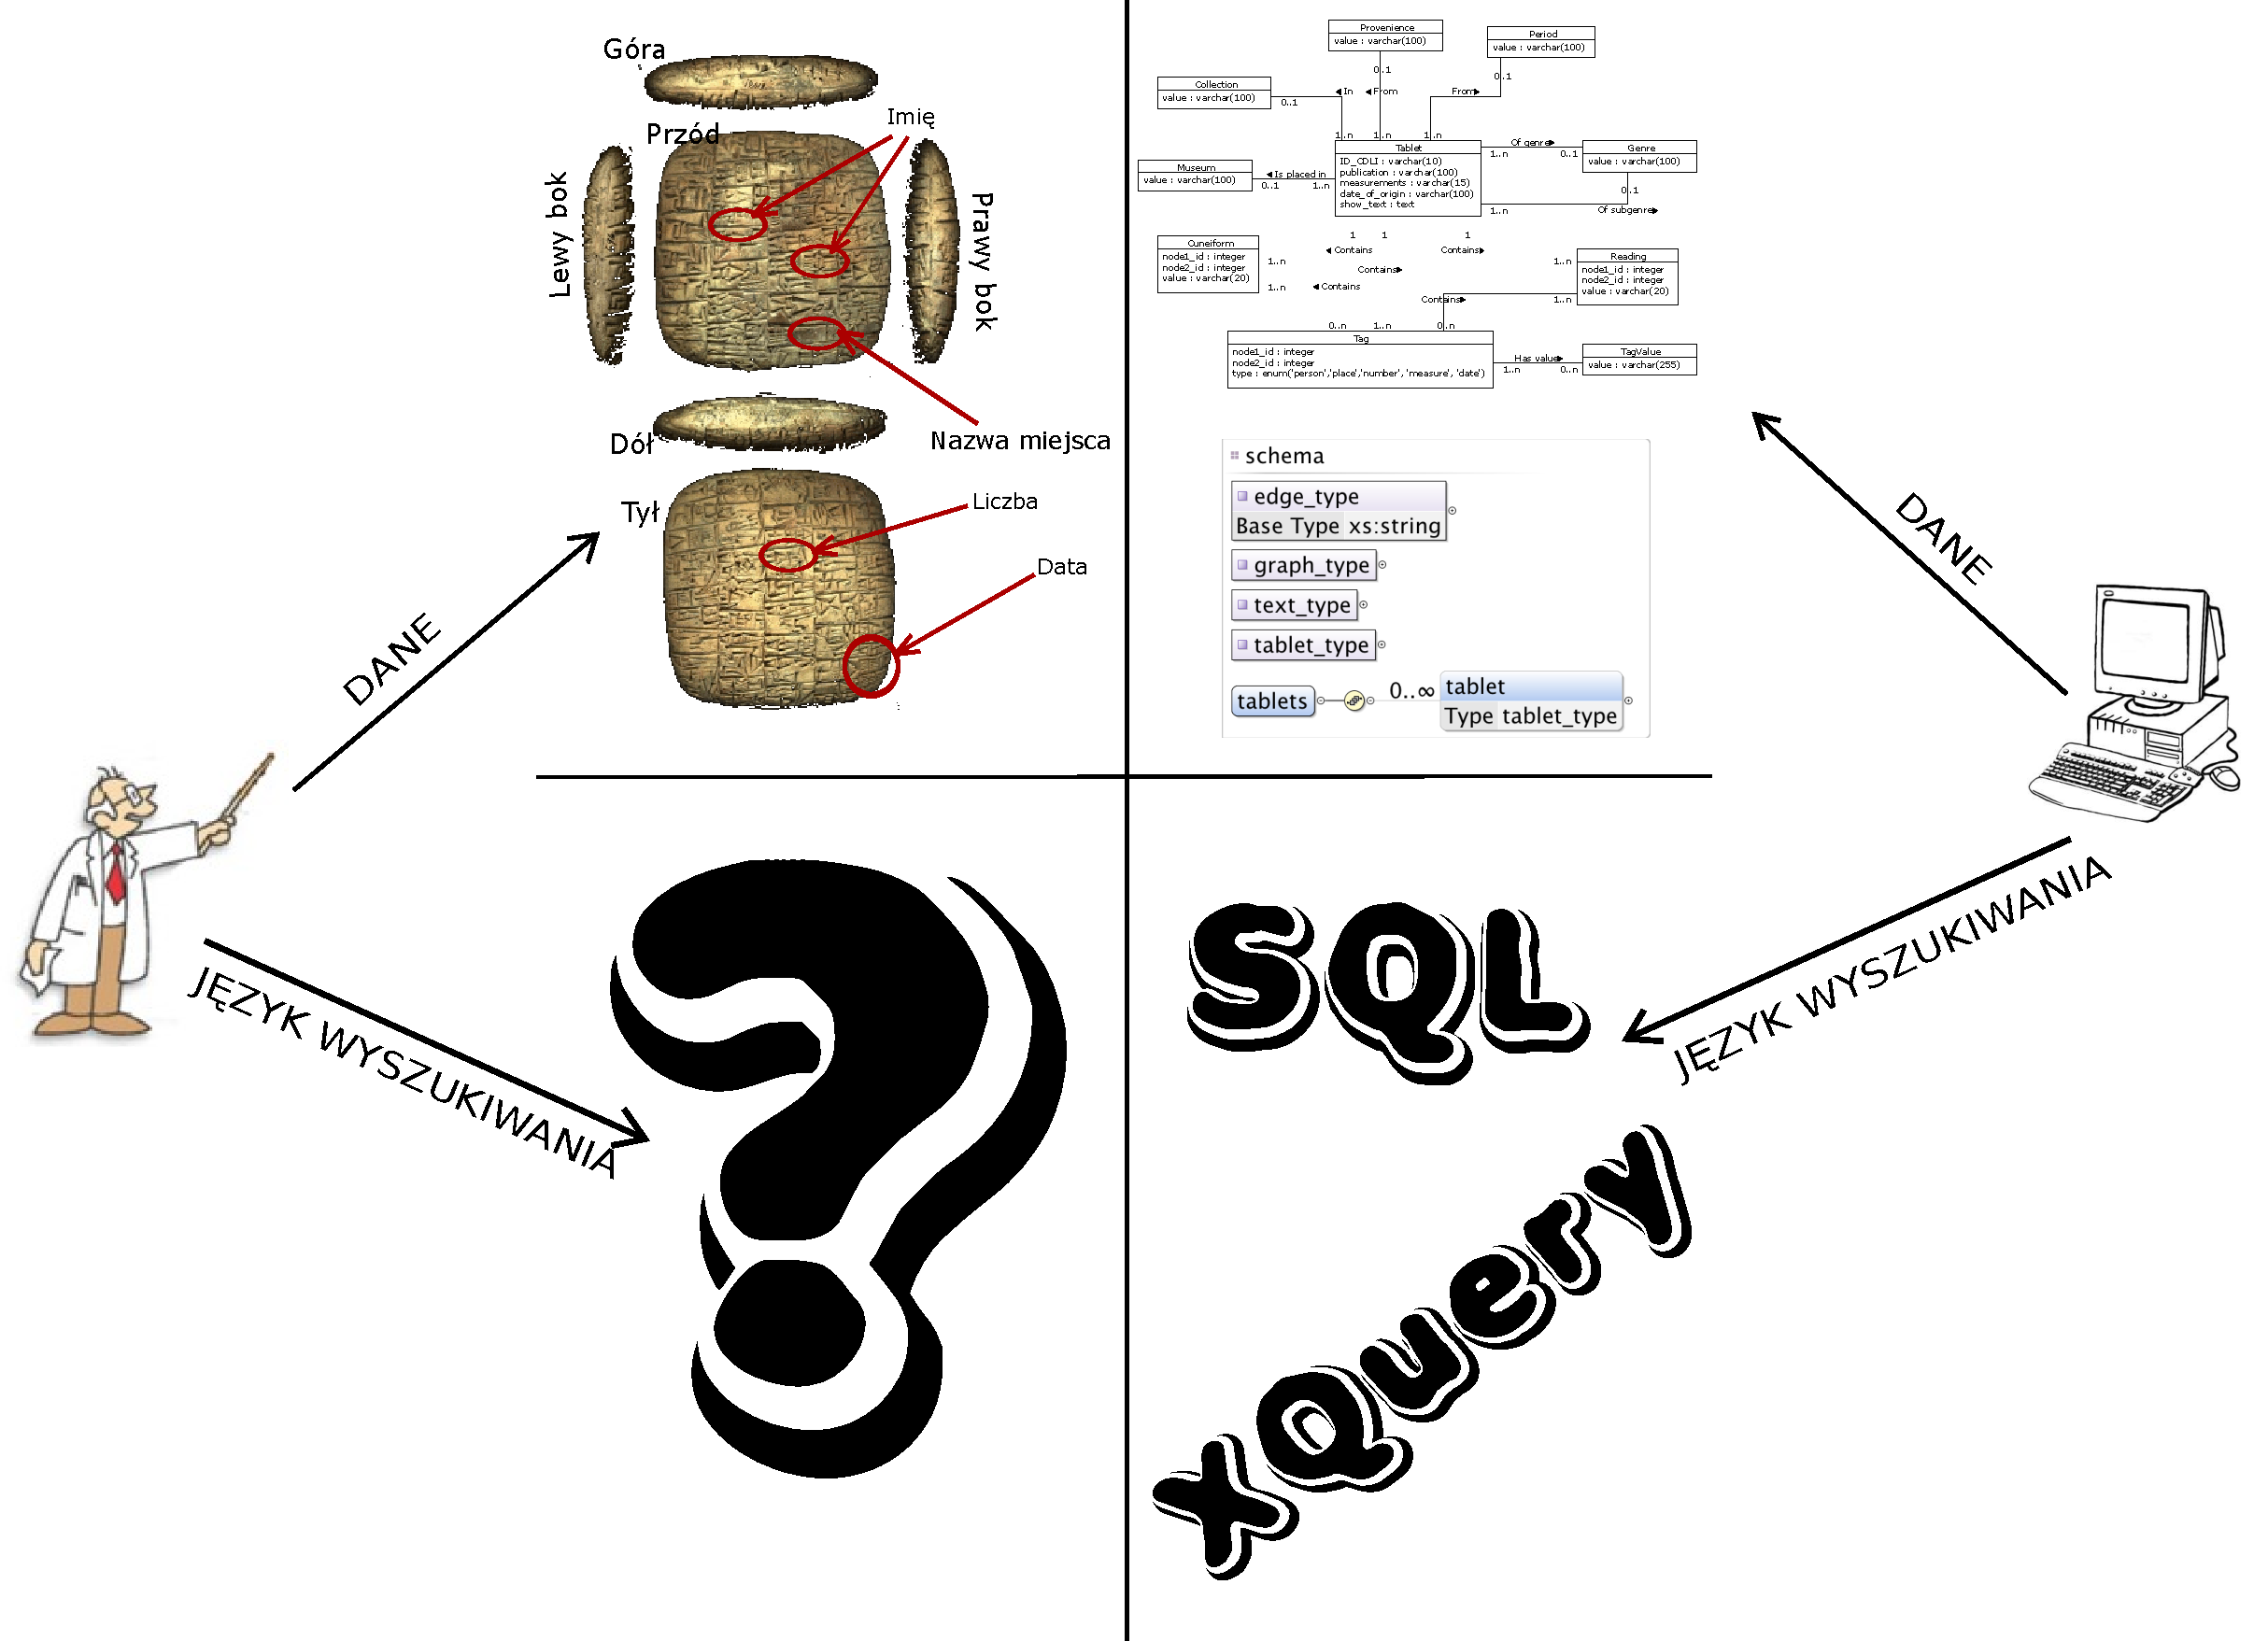
\includegraphics[width=365px]{./diagramy/poco.pdf}
 
 
Niniejsza praca dotyczy problemu przetwarzania baz danych tabliczek sumeryjskich przez osoby nieznające specyficznych dla baz danych języków zapytań.

Istnieje wiele baz danych zawierających teksty odczytane z tabliczek sumeryjskich (najbardziej znana - CDLI zawiera prawie 225 tys. tekstów). Sumerolodzy zajmują się badaniem i przetwarzaniem tych tekstów, jednak wyszukiwanie interesujących ich tabliczek wciąż stanowi dla nich problem. Jest to spowodowane przede wszystkim nieznajomością specyficznych dla baz danych języków zapytań. W celu rozwiązania tego problemu wiele serwisów udostępnia formularze służące do wyszukiwania, ale mają one ograniczone możliwości. Dlatego istnieje potrzeba stworzenia narzędzia, które będzie łączyło w sobie jak największą siłę wyrazu i łatwość użycia przez osoby znające jedynie dziedzinę problemu. Takim narzędziem jest zaprojektowany przez nas język TQL. 


Istnieją też inne grupy ludzi potrzebujące podobnego języka (np. językoznawcy). 
Większość programów ułatwiających tworzenie zapytań jest skomplikowana, daje ograniczone możliwości lub jest przystosowana głównie do przetwarzania danych liczbowych. Tablets Query Language rozwiązuje te problemy: jest prosty i intuicyjny, przystosowany głównie do tekstów, minimalnie zmniejsza siłę wyrazu oraz łatwo go rozbudowywać. 

%Język TQL jest nakładką na inne języki (m.in. SQL). 
TQL jest jednym z języków dziedzinowych (Domain Specific Languages, DSL). 
W związku z tym dla każdego sposobu reprezentacji danych należy skonstruować translator, 
którego zadaniem będzie przetłumaczenie zapytania. 
% Dla każdego z nich, w zależności od reprezentacji danych, należy skonstruować translator, 
% którego zadaniem będzie przetłumaczenie zapytania. 
W ramach niniejszej pracy przedstawione zostaną dwa przykładowe translatory.
